\documentclass{article}
\usepackage{graphicx}
\usepackage[margin=1.5cm]{geometry}
\usepackage{amsmath}

\begin{document}

\title{Warm Up: Graphical Analysis of Kinematics}
\author{Prof. Jordan C. Hanson}

\maketitle

\section{Memory Bank}

\begin{enumerate}
\item $v = \frac{\Delta x}{\Delta t}$ ... Average velocity.
\item $x(t) = v t + x_i$ ... Position versus time with constant velocity.
\item $a = \frac{\Delta v}{\Delta t}$ ... Acceleration is the change in velocity.
\item $v_f^2 = v_i^2 + 2 a \Delta x$ ... Kinematic equation without time.
\end{enumerate}

\section{Graphical Analysis of Kinematics}

\begin{figure}[ht]
\centering
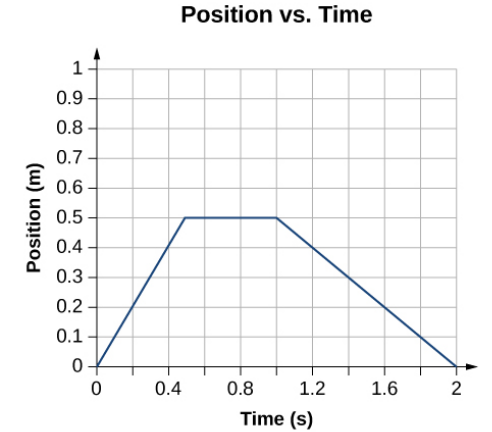
\includegraphics[width=0.25\textwidth]{figures/x_vs_t.png} \hspace{0.5cm}
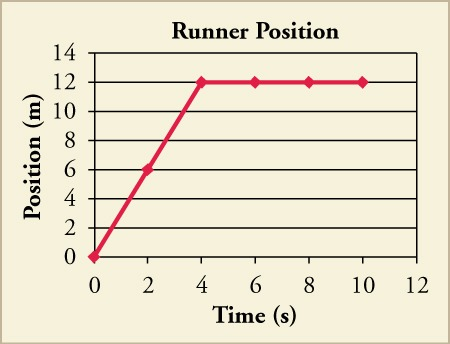
\includegraphics[width=0.25\textwidth]{figures/run.jpeg}
\caption{\label{fig:graph} (Left) A graph of the displacement versus time of a system, in meters versus seconds. (Right) A graph of displacement versus time of a runner, in meters versus seconds.}
\end{figure}

\begin{enumerate}
\item Consider Fig. \ref{fig:graph} (Left).  (a) What is the velocity of the system between 0 and 0.5 seconds? (b) What is the velocity between 0.5 and 1.0 seconds? (c) What is the velocity between 1.0 and 2.0 seconds? \\ \vspace{0.5cm}
\item Write the formula $x(t)$ that describes the motion between 1.0 and 2.0 seconds. \\ \vspace{0.5cm}
\item Consider the motion of the runner depicted in Fig. \ref{fig:graph} (Right).  (a) What is the speed of the system after $t = 4$ seconds? (b) What is the acceleration between $t=0$ and $t=4$ seconds? (c) What is the speed of the runner between $t=0$ and $t=4$ seconds? \\ \vspace{1cm}
\item Now change the y-axis units in Fig. \ref{fig:graph} to velocity, in meters per second.  Answer parts (a)-(c) from the previous question again.  For part (c), write your answer as a function of time.  \textit{Where} does the runner reach top speed? \\ \vspace{1cm}
\end{enumerate}

\end{document}
